\documentclass[11pt]{article}
\usepackage[margin=0.85in]{geometry}
\usepackage{times}
\usepackage{graphicx}
\usepackage{tikz}
\usepackage{pgfplots}
\usepackage{booktabs}
\usepackage{hyperref}
\usepackage{enumitem}
\usepackage{xcolor}
\usepackage{caption}
\pgfplotsset{compat=1.18}
\usetikzlibrary{arrows.meta,positioning,fit,calc}

\hypersetup{colorlinks=true,linkcolor=black,urlcolor=blue!50!black,citecolor=black}
\pagestyle{plain}
\setlist[itemize]{leftmargin=1.2em,itemsep=0.15em,topsep=0.2em}
\setlist[enumerate]{leftmargin=1.2em,itemsep=0.15em,topsep=0.2em}
\captionsetup{font=small, skip=6pt}

\title{\vspace{-1.2em}\bfseries Hypothesis-Tree Molecular Agents for GuacaMol Amlodipine MPO}
\author{\vspace{-0.4em}Research Proposal \\[0.2em]
\small Ashutosh Ganguly and collaborators \\
\small Tree AI Scientist / autonomous molecular discovery}
\date{\vspace{-0.6em}\small October 2026}

\begin{document}
\maketitle
\vspace{-1.2em}

\section{Introduction}
GuacaMol's \textbf{Amlodipine MPO} asks an agent to propose molecules that score highly under a black-box multi-property objective built around similarity to the antihypertensive drug Amlodipine and a preferred ring count. The formula is withheld from the agent: it only sees SMILES strings and numeric scores. Classical generative baselines often burn tens of thousands of oracle calls; our premise is that a \emph{scientific} agent---one that reads, hypothesizes, experiments, and writes---can climb the same landscape with far fewer evaluations.

We cast discovery as a \textbf{hypothesis tree}. Each \emph{node} is a hypothesis experiment that ends in a short research paper (methods, measured matrix, observation, conclusion). Each \emph{edge} is temporal: a child is proposed after its parent is committed, so the tree is an explicit, searchable laboratory notebook rather than a flat list of samples. A single LLM (Qwen) rotates through controller, planner, observer, and reporter roles, using tools to browse memory and submit structured actions. On our Amlodipine campaign the incumbent rose from a seed score of $\mathbf{0.368}$ to $\mathbf{0.905}$ in \textbf{83} oracle calls and \textbf{48} papers---evidence that autonomous scientific loops can be both sample-efficient and chemically meaningful.

\begin{figure}[t]
\centering
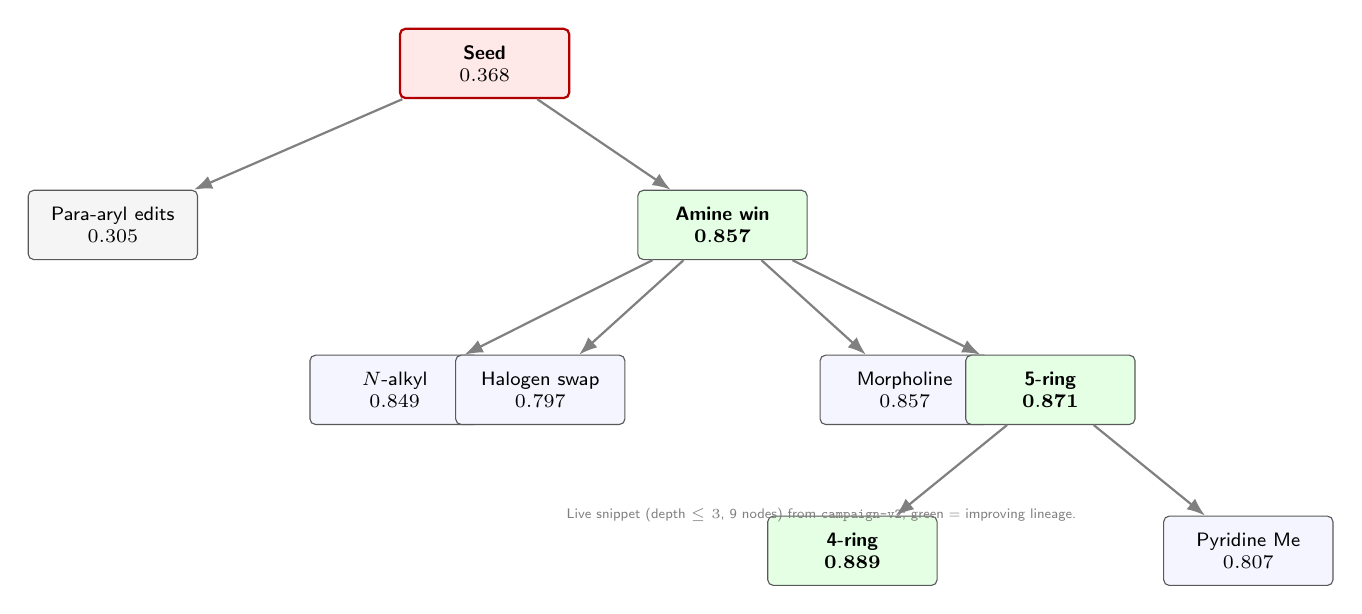
\begin{tikzpicture}[
  font=\scriptsize\sffamily,
  every node/.style={align=center},
  box/.style={draw=black!65, rounded corners=2pt, inner sep=3pt, fill=white,
              minimum width=2.15cm, minimum height=0.88cm},
  root/.style={box, draw=red!70!black, fill=red!9, thick},
  win/.style={box, fill=green!10},
  mid/.style={box, fill=blue!4},
  bad/.style={box, fill=black!4},
  edge/.style={-{Latex}, thick, black!50},
  level distance=1.35cm,
  sibling distance=2.35cm
]
\node[root] (r) {\textbf{Seed}\\$0.368$};
\node[bad, below left=1.15cm and 2.55cm of r] (a) {Para-aryl edits\\$0.305$};
\node[win, below right=1.15cm and 0.85cm of r] (b) {\textbf{Amine win}\\$\mathbf{0.857}$};
\node[mid, below left=1.2cm and 2.0cm of b] (c1) {$N$-alkyl\\$0.849$};
\node[mid, below left=1.2cm and 0.15cm of b] (c2) {Halogen swap\\$0.797$};
\node[mid, below right=1.2cm and 0.15cm of b] (c3) {Morpholine\\$0.857$};
\node[win, below right=1.2cm and 2.0cm of b] (c4) {\textbf{5-ring}\\$\mathbf{0.871}$};
\node[win, below left=1.15cm and 0.35cm of c4] (d1) {\textbf{4-ring}\\$\mathbf{0.889}$};
\node[mid, below right=1.15cm and 0.35cm of c4] (d2) {Pyridine Me\\$0.807$};
\draw[edge] (r) -- (a);
\draw[edge] (r) -- (b);
\draw[edge] (b) -- (c1);
\draw[edge] (b) -- (c2);
\draw[edge] (b) -- (c3);
\draw[edge] (b) -- (c4);
\draw[edge] (c4) -- (d1);
\draw[edge] (c4) -- (d2);
\node[font=\tiny\sffamily, text=black!50, below=0.35cm of $(c1)!0.5!(d2)$]
  {Live snippet (depth $\leq 3$, 9 nodes) from \texttt{campaign-v2}; green = improving lineage.};
\end{tikzpicture}
\caption{Hypothesis tree from the Amlodipine run. The red root is the seed; green nodes track the rising incumbent through depth~3.}
\label{fig:tree}
\end{figure}

\section{Action space}
The agent never free-forms tool calls in prose. Every turn returns one JSON envelope \texttt{\{reason, action, args\}}. The edited memory and decision surface we emphasize is:

\begin{itemize}
  \item \texttt{inspect\_tree} --- paginated gists (title, best molecule, outcome).
  \item \texttt{read} / \texttt{search} / \texttt{compare} --- paper chunks, hybrid retrieval, multi-node facts.
  \item \texttt{deep\_read} --- dedicated reader model; saves a note (not the raw paper dump).
  \item \texttt{select\_parent} / \texttt{propose\_hypotheses} --- pick a line of work; spawn two sibling claims.
  \item \texttt{submit\_matrix} --- freeze bases$\times$strategies candidates (oracle runs \emph{after} both siblings plan).
  \item \texttt{submit\_paper} --- commit the experiment paper into the git-backed archive.
\end{itemize}

\noindent Figure~\ref{fig:actions} shows how often these actions fired on the thinking-on Amlodipine campaign. Memory browsing dominates early; matrix and paper submits track the 48 completed experiments.

\begin{figure}[t]
\centering
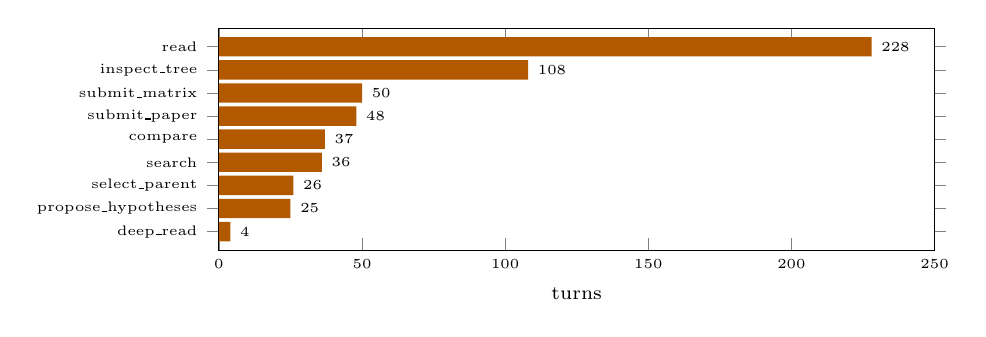
\begin{tikzpicture}
\begin{axis}[
  xbar,
  width=0.88\linewidth, height=4.4cm,
  xmin=0, xmax=250,
  symbolic y coords={deep\_read,propose\_hypotheses,select\_parent,search,compare,submit\_paper,submit\_matrix,inspect\_tree,read},
  ytick=data,
  nodes near coords, nodes near coords align={horizontal},
  every node near coord/.append style={font=\tiny},
  xlabel={turns},
  tick label style={font=\tiny},
  label style={font=\scriptsize},
  bar width=7pt,
]
\addplot[fill=orange!70!black, draw=none] coordinates {
  (4,deep\_read) (25,propose\_hypotheses) (26,select\_parent)
  (36,search) (37,compare) (48,submit\_paper) (50,submit\_matrix)
  (108,inspect\_tree) (228,read)
};
\end{axis}
\end{tikzpicture}
\caption{Edited action histogram (thinking-on Amlodipine).}
\label{fig:actions}
\end{figure}

\section{An agent's trajectory}
A concrete path from the live tree:

\begin{enumerate}[leftmargin=1.4em]
  \item \textbf{Level 0 (root).} Seed with Amlodipine itself (score $0.368$). Chemically relevant, but not optimal under the ring-aware objective.
  \item \textbf{Level 1.} Para-aryl bulk fails ($0.305$). Replacing the terminal primary amine with a piperazinyl side chain \textbf{jumps to $0.857$}.
  \item \textbf{Level 2.} Children fence that win; shrinking the distal diamine toward a five-membered ring lifts the incumbent to $\mathbf{0.871}$.
  \item \textbf{Levels 3--4.} Further ring compression (4-membered, then 3-membered diazacyclopropane) reaches $\mathbf{0.905}$.
  \item \textbf{Deeper levels.} Later papers mostly defend the optimum with near-neighbors and controls.
\end{enumerate}

\begin{figure}[t]
\centering
\includegraphics[width=0.98\linewidth]{figs/mol_evolution.png}\\[0.35em]
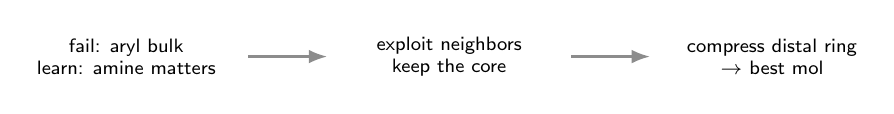
\begin{tikzpicture}[font=\scriptsize\sffamily, every node/.style={align=center}]
  \node (a) at (0,0) {fail: aryl bulk\\learn: amine matters};
  \node (b) at (4.1,0) {exploit neighbors\\keep the core};
  \node (c) at (8.2,0) {compress distal ring\\$\rightarrow$ best mol};
  \draw[-{Latex}, thick, black!45] (1.55,0) -- (2.55,0);
  \draw[-{Latex}, thick, black!45] (5.65,0) -- (6.65,0);
\end{tikzpicture}
\caption{Molecule evolution along the winning lineage (structures, not SMILES): seed $\rightarrow$ L1 amine win $\rightarrow$ L2 five-membered distal ring $\rightarrow$ best three-membered ring ($0.368\rightarrow0.857\rightarrow0.871\rightarrow0.905$), with the learnings that drove each hop.}
\label{fig:mols}
\end{figure}

\section{Conclusion: what improved}
Starting from Amlodipine ($0.368$), the agent discovered that the under-scoring axis was largely the \textbf{terminal amine / distal ring geometry}, not the pyridine diester core. Keeping that body and installing a compact three-membered diazacyclopropane on the side chain lifted the score to $\mathbf{0.905}$ after only $\mathbf{83}$ black-box calls. That is the collaboration hook: \textbf{autonomous agents that write real experimental memory can design better molecules at a fraction of the usual oracle budget}, and every step remains inspectable as a paper in a tree.

\section*{Open questions}
\begin{enumerate}[leftmargin=1.4em]
  \item \textbf{Steering tool use with SFT / RL.} Figure~\ref{fig:actions} shows a strong bias toward \texttt{read}/\texttt{inspect\_tree}. Can preference optimization or process rewards reshape this histogram---more targeted \texttt{search}/\texttt{deep\_read}, fewer redundant pages---without hurting chemical progress?
  \item \textbf{Deeper thinking, richer search.} Beyond document tools, we want better tree-search algorithms and actions such as \texttt{think\_more} or \texttt{try\_a\_bigger\_oracle\_call}, so the agent can deliberate longer, spend budget when uncertainty is high, and plan across many papers rather than reacting turn-by-turn.
\end{enumerate}

\end{document}
